\documentclass{ci5652}
\usepackage{graphicx,amssymb,amsmath}
\usepackage[utf8]{inputenc}
\usepackage[spanish]{babel}
\usepackage{hyperref}
\usepackage{subfigure}
\usepackage{paralist}
\usepackage[ruled,vlined,linesnumbered]{algorithm2e}
\usepackage{graphicx}
\graphicspath{ {images/} }

%----------------------- Macros and Definitions --------------------------

% Add all additional macros here, do NOT include any additional files.

% The environments theorem (Theorem), invar (Invariant), lemma (Lemma),
% cor (Corollary), obs (Observation), conj (Conjecture), and prop
% (Proposition) are already defined in the ci5652.cls file.

%----------------------- Title -------------------------------------------

\title{Desarrollo y Evaluación de Metaheurísticas para el Problema de Asignación Cuadrática}

\author{Luis Fernandes (lfernandes@ldc.usb.ve)
        \and
        Donato Rolo (donato@ldc.usb.ve)}





%------------------------------ Text -------------------------------------

\begin{document}
\thispagestyle{empty}
\maketitle
\begin{abstract}

Muchos son los algoritmos y las metaheurísticas diseñadas a lo largo del tiempo para encontrar la solución óptima al problema de asignación cuadrática, el cual es un problema NP-duro como bien demuestran Sahni y González en \cite{sahni1976}, para nuestros propósitos, se buscará desarrollar distintas metaheurísticas sobre este problema para luego evaluarlas y compararlas, así como también se evaluarán distintas formas de desarrollar los componentes de tales metaheurísticas, tales como las soluciones iniciales generadas, las vecindades de las soluciones propuestas, entre otros. 
.
\end{abstract}

\section{Introducción}

El problema de asignación cuadrática, fue presentado por Koopmans y Beckmann en 1957 \cite{koopmans1957} como un modelo matemático para la ubicación de un conjunto actividades económicas.
Es uno de los problemas de optimización combinatoria fundamental, usualmente es utilizado para describir un problema de ubicación.

Se considera el problema de asignación como un conjunto de ubicaciones, donde se toma en cuenta el costo como una función entre la distancia y flujo entre las facilidades. El objetivo principal es minimizar el costo total, ubicando cada facilidad en la localización que cumpla dicho objetivo.

Entre las aplicaciones que se le pueden atribuir al problema de asignación cuadrática se puede encontrar el diseño de terminales de aeropuertos, en donde se quiere que los pasajeros que deban hacer un transbordo recorran la distancia mínima entre una y otra terminal, teniendo en cuenta el flujo de personas entre ellas, procesos de comunicaciones y diseño de circuitos eléctricos, en donde es de relevante importancia dónde se ubican ciertas partes o chips con el fin de minimizar la distancia entre ellos, ya que las conexiones son de alto costo, entre otras.

El presente artículo está estructurado de la siguiente forma: primero se indicará la formulación matemática propuesta para el problema, luego se especificará un algoritmo de búsqueda local cuyo objetivo es encontrar soluciones mejores hasta quedarse en algún mínimo local, tal búsqueda local dependerá de factores muy fundamentales como son la producción de una solución inicial y la vecindad de soluciones a generar, tales puntos también serán cubiertos; posteriormente, se propondrán dos metaheurísticas que buscan escapar de los mínimos locales que produce el \textit{Local Search} y de esta forma abrir el espacio de búsqueda para encontrar nuevas y mejores soluciones, tales metaheurísticas son las de \textit{Iterated Local Search} y \textit{Tabu Search} su estructura general, componentes principales y detalles de implementación propuesta serán especificados. Posteriormente, se presentarán dos opciones de metaheurísticas poblacionales que son sustancialmente diferentes a las metaheurísticas de trayectoria anteriormente mencionadas. Las metaheurísticas poblacionales escogidas para el presente artículo son \textit{Genetic Algorithm} y \textit{Scatter Search}. Finalmente, se expondrán los resultados de las evaluaciones de tales metaheurísticas con su respectivo análisis y de esta forma tomarán conclusiones al respecto en la última sección. 

\section{Formulación Matemática}

Para el problema de asignación cuadrática existen varias modelaciones y formulaciones, sin embargo nosotros nos hemos basado en la formulación propuesta por Koopman y Beckman en \cite{koopmans1957} y la propuesta en la librería de instancias de Burkard et al. \cite{burkard2012}, en el cual se busca una combinación de las facilidades en las localizaciones propuestas tal que

\[min_{p\in \prod I_{n}} \sum_{i}^{n}\sum_{j}^{n}f_{i,j}d_{p(i,j)}\]

Donde \(I_{n}\) es el conjunto de los números pertenecientes al intervalo [1..n], \(\prod I_{n}\) son todas las permutaciones de tal conjunto, \(f_{i,j}\) es el flujo de la facilidad \(i\) a la facilidad \(j\) y \(d_{p(i,j)}\) es la distancia de la localización asignada a la facilidad \(i\) a la localización asignada a la locaclización \(j\). Por tal formulación, las soluciones propuestas son representadas como \(S = {s_{1}}, s_{2}, ..., s_{n}\), donde cada \(s_{i}\) es la localización asignada a la facilidad \(i\).


\section{Búsqueda Local}

  Para la búsqueda local de este problema, se realizó la propuesta de obtener una solución inicial basada en un algoritmo greedy, una vez obtenida una solución se obtendrán nuevas vecindades de la última mejor solución a través de un operador y se evaluará por completo tal vecindad, una vez tomada una mejor solución de tal vecindad, se realizará de nuevo la búsqueda hasta que no se pueda encontrar una mejor solución o se llegue a la condición de parada. Basado en esto, el algoritmo de búsqueda local se puede representar de la siguiente manera:
    
\begin{algorithm}
 \DontPrintSemicolon
 \vspace*{0.1cm}
 %\KwIn{Descripcion}
 %\KwOut{Descripcion}
 s $\leftarrow$ greedy()\;
 \While{$\neg$condiciónDeParada()}{
  $N(S) \leftarrow generarVecindad(S)$\;
  $S' \leftarrow obtenerMejor(N(S))$\;
  \eIf{c(S')\textless c(S)}{
   S = S'\;
   }{
  \KwRet{S}\;  
   }
 }
 
 \KwRet{S}
 \vspace*{0.1cm}
 \caption{Búsqueda Local}
\end{algorithm}
    
  Donde \(obtenerMejor(N(S))\) simplemente evalúa cada elemento de tal conjunto y obtiene aquel cuya función de evaluación sea la menor, \(c(S)\) es el resultado obtenido de tal función de evaluación en una solución \(S\) y la condición de parada puede variar, en nuestro caso se ha implementado una condición de parada basada en el número de iteraciones el cual se ha colocado con una cota máxima de veinte iteraciones. Esta cota superior aunque parezca bastante estricta, el operador de vecindad utilizado genera una vecindad bastante moderada tanto en cardinalidad como en pluralidad de la solución, este operador será descrito más adelante. 
  
  Una posible variación al problema surge cambiando por completo la solución inicial, de una solución obtenida a través de un algoritmo Greedy se puede obtener también una solución inicial a través de una generación de secuencia totalmente aleatoria, la cual también será descrita en una sección más adelante.

\subsection{Greedy}

Una de las dos posibles soluciones iniciales a generar la hemos realizado a través de un algoritmo greedy que a groso modo busca darle las mejores ubicaciones a las facilidades con mayor flujo, para esto se debe obtener el flujo total de cada \(f_{i}\in F\), donde \(F\) es el conjunto de todas las facilidades, para obtener tal flujo total, se deben sumar el flujo de esta facilidad con cada una de las otras facilidades, es decir, cada facilidad \(k\) posee un \(f_{k total} = \sum_{i=1}^{n}f_{k,i}\), de forma similar, cada localización posee una distancia total, que es la suma de las distancias a las otras localizaciones, o lo que es igual, cada localización \(k\) tiene una suma de distancias \(d_{k total} = \sum_{i=1}^{n}d_{k,i}\). Con estos valores de flujo y distancia total para cada facilidad y localización respectivamente, se ordenan a las facilidades y a las localizaciones de forma ascendente, luego se procede a realizar la asignación de forma tal que para la i - ésima facilidad se le asigne la n - i-ésima localización. El algoritmo se presenta a continuación:

\begin{algorithm}
 \DontPrintSemicolon
 \vspace*{0.1cm}
 \KwIn{n: tamaño de las matrices, F: Matriz de Flujo, L: Matriz de localizaciones}
 \KwOut{S: Solución inicial}
 \For{cada $f_{i}$ $\in$ F}{
  $facilidades_{i} \leftarrow$ \textless $f_{i}, flujoTotal(f_{i})$\textgreater\;
 }
 ordenarPorFlujoTotal(flujos)\;
 \For{cada $l_{i}$ $\in$ L}{
  $localizaciones_{i} \leftarrow$ \textless $l_{i}, distanciaTotal(f_{i})$\textgreater\;
 }
 ordenarPorDistanciaTotal(localizaciones)\;
 \For{i $\in$ \{1..n\}}{
  $S_{facilidades_{n-i}} \leftarrow localizaciones_{i}$\;
 }
 
 
 \KwRet{S}
 \vspace*{0.1cm}
 \caption{QAP Greedy}
\end{algorithm}
    

De este algoritmo se tiene que tanto el procedimiento \(ordenarPorDistanciaTotal\) como el procedimiento \(ordenarPorFlujoTotal\) ordenan la secuencia que reciben como entrada de forma ascendente según la distancia total o el flujo total de sus componentes según corresponda. Por otro lado, las funciones \(flujoTotal\) obtiene el flujo total de la facilidad que es pasada como parámetro a la función, mientras que la función \(distanciaTotal\) obtiene la distancia total de un localización.



\subsection{Random}

Esta alternativa a solución inicial es simplemente una asignación aleatoria de cada localización a una facilidad en particular, el uso de esta solución inicial es simplemente para la evaluación de esta alternativa frente a la solución Greedy.  

\section{Vecindad}

Para la generación de vecindades se ha propuesto un operador muy particular, escogido básicamente por sus propiedades de generación de soluciones desiguales y por la cardinalidad del conjunto de vecindad que genera. El operador de vecindad al cual denominaremos "rotate and swap" a partir de ahora consta de dos fases como su nombre lo indica, la primera está basada en ir rotando el conjunto solución, la segunda de ir haciendo cambios de los elementos desde la primera posición con el elemento de la última, luego intercambia el segundo elemento con el antepenúltimo, y así sucesivamente hasta generar una solución palíndroma a la solución resultante de la rotación, cabe destacar que todas las soluciones intermedias producto de los intercambios son guardadas en el conjunto vecindad resultante.

De esta forma es posible identificar el conjunto vecindad de una solución \(S =\) \textless \(a_{1}, a_{2}, ..., a_{n}\)\textgreater \space (con \(n\) siendo el tamaño de tal secuencia) como la unión del conjunto rotación con el conjunto de swaps de cada rotación, es decir \(R\) U \(SW\), donde:
\newline
\(R = \{\)\textless \(a_{(1+i) mod n}, a_{(2+i) mod n}, ..., a_{(n+i) mod n}\)\textgreater \( \| i\in\{ 1, 2, ..., n\} \}\) 
\newline
y 
\newline
\(SW = \{ \)\textless \(a_{1}, a_{2}, ..., a_{n-i+1}, ..., a_{i}, ..., a_{n-1}, a_{n}\)\textgreater \( \| i\in\{ 1, 2, ..., n/2\} \wedge \forall x\in R \}   \)
\newline
Bajo este operador de vecindad se obtienen exactamente \(n^{2}/2\) distintas, \(n\) obtenidas por las rotaciones de la solución inicial y \(n/2\) para cada una de las soluciones generadas por la rotación debido al swap provisto.


\section{Metaheurísticas de Trayectoria}

Para el Problema de Asignación Cuadrática hay varias metaheurísticas que se han desarrollado para la obtención de soluciones óptimas como para la obtención de buenos resultados para problemas en los cuales el espacio de búsqueda es extensamente abrumador. Tales son los casos de Thomas Stützle con su alternativa de \textit{Iterated Local Search} con criterios de aceptación y \textit{history} \cite{stutzle1999}, un \textit{Simulated Annealing} propuesto por Ghandeshtani et al. \cite{ghandeshtani2010}, un \textit{Tabu Search} de Taillard \cite{taillard1991}, e incluso algunas combinaciones de metaheurísticas como la propuesta por Misevicius et al. \cite{misevicius2006} en el cual aplican una especie de \textit{Tabu Search} iterativo. 

Para nuestros efectos nos hemos propuesto desarrollar dos metaheurísticas de trayectoria para luego evaluarlas y compararlas, el desarrollo de las mismas será especificado en las subsecciones a continuación, la evaluación y comparación será dejada para una sección de evaluación más adelante.

\subsection{Iterated Local Search}

El \textit{Iterated Local Search} es una metaheurística que busca salir de óptimos locales a través de la diversificación del espacio de búsqueda, como bien explica Stützle en \cite{stutzle1999}, el algoritmo se enfoca en realizar búsquedas locales y cuando ya no logre encontrar algo mejor se perturba la solución para luego realizar una búsqueda local sobre dicha nueva solución y realizar esto un número determinado de veces, posteriormente la mejor solución encontrada durante todo el procedimiento debió haber sido guardada para identificarla.

En nuestro caso hemos implementado un \textit{Iterated Local Search} con características muy propias, se comienza con la solución propuesta en §4, y luego se obteniene el mínimo local aplicando el algoritmo de la §3, de esta forma, independientemente de cuantas veces se realice este algoritmo o de cuantas iteraciones se plantee, al menos conseguirá una solución tan buena como la que encuentre de aplicar un Local Search sobre la solución inicial generada por el Greedy especificado anteriormente. Posteriormente, se generarán otras soluciones completamente aleatorias (lo cual sería parte de la perturbación) y utilizando §3 se obtiene un nuevo mínimo local y se compara con la mejor solución que se haya obtenido para ver si esta última es mejor. Este procedimiento se ejecuta un número arbitrario de veces, 20 mil en nuestro caso dado que es el número de iteraciones con el que hemos conseguido buenos resultados y no es exhaustivo en el consumo de tiempo, la condición de parada también especifica que si se han cumplido 2 mil iteraciones (una décima parte del total) sin encontrar una nueva mejor solución se debe detener la búsqueda, esto para evitar un iteraciones inútiles.


\begin{algorithm}
 \DontPrintSemicolon
 \vspace*{0.1cm}
 %\KwIn{Descripcion}
 %\KwOut{Descripcion}
 S* $\leftarrow$ greedy()\;
 S $\leftarrow$ S*\;
 \While{$\neg$condiciónDeParada()}{
 
  $S \leftarrow localSearch(S)$\;

  \eIf{f(S) \textless f(S*)}{
    S* $\leftarrow$ S\;
   }{
    skip\;
   }
  S $\leftarrow$ randomSolution()\;
 }
 
 \KwRet{S*}
 \vspace*{0.1cm}
 \caption{Iterated Local Search}
\end{algorithm}

\subsection{Tabu Search}

El \textit{Tabu Search} es una metaheurística que puede ser implementada con distintas variaciones y distintos sabores, sin embargo hay ciertas características que deben estar presentes, como la \textit{lista Tabu}, en la cual se almacenan los movimientos previamente realizados para llegar a la solución actual y cuyo propósito es tener información de estos movimientos para evitar realizarlos nuevamente y escapar de mínimos locales aceptando soluciones que no sean obtenidas a través de tales movimientos, de esta forma se garantiza un mayor espacio de búsqueda que en el efectuado por el \textit{Local Search}, el cual se queda con el primer mínimo local que llegue a encontrar. 

Para nuestros efectos, nos hemos propuesto en desarrollar un \textit{Tabu Search} con \textit{memoria estática} de tamaño \(n\), el tamaño de esta lista es de vital importancia, puesto que con un tamaño demasiado pequeño no se evita buen espacio de búsqueda pero a la vez con un tamaño muy grande se puede estar evitando demasiado espacio de búsqueda, tras realizar algunas pruebas concordamos con fijar este tamaño en \(n\), por los posibles movimientos que puede almacenar, el cual depende en gran medida del operador para generación de vecindad utilizado, que para este caso en particular se ha utilizado el operador de \(2-exchange operator\), como lo describen Koopmans y Beckmann \cite{koopmans1957}, el cual genera una vecindad de una secuencia \textit{a} a partir de todos los cambios posibles de pares de elementos de tal secuencia, bajo este operador se pueden obtener \(n*(n-1)/2\) soluciones nuevas y con una lista de tabu de tamaño \(n\) se evita una buena pero prudente fracción de tal espacio de búsqueda (en caso de que la lista se encuentre llena). Esta lista se comporta como una cola, en la cual si el tamaño de la lista ha alcanzado el tope y hay que almacenar un nuevo movimiento, la cola deshecha el movimiento más antiguo introducido. Aún así es posible realizar un movimiento de la lista Tabu sobre la solución actual, pero esto solo es posible si y solo si tal movimiento permite llegar a una solución que es mejor a cualquier otra solución previamente vista.

Nuestro algoritmo tabu evalúa toda la vecindad generada para ver las mejores soluciones de tal vecindad, de haber una mejor solución a cualquier vista previamente se toma sin importar que el movimiento que la genere se encuentre en la lista tabú o no como se explicó hace un momento, de no haber tal solución se procede a tomar la mejor de la vecindad que no se encuentre en la lista tabu, sin importar si tal solución es mejor que la actual, de hecho es la forma de escapar del mínimo local. Es importante señalar que como solución inicial se ha escogido el método de solución inicial aleatoria. El algoritmo se muestra a continuación.

\begin{algorithm}
 \DontPrintSemicolon
 \vspace*{0.1cm}
 %\KwIn{Descripcion}
 %\KwOut{Descripcion}
 S* $\leftarrow$ randomSolution()\;
 S $\leftarrow$ S*\;
 \While{$\neg$condiciónDeParada()}{
  $N(S) \leftarrow generarVecindad(S)$\;
  $S' \leftarrow obtenerMejor(N(S))$\;
  \eIf{f(mejorSolución(N(S))) \textless f(S*)}{
   S* $\leftarrow$ mejorSolución(N(S))\;
   }{ 
   S $\leftarrow$ mejorSolución(N(S)$\backslash$LT)\;
   }
  actualizaLT()\;
 }
 
 \KwRet{S*}
 \vspace*{0.1cm}
 \caption{Tabu Search}
\end{algorithm}

En el anterior algoritmo el procedimiento mejorSolución() simplemente devuelve la mejor solución del conjunto que le sea pasado como entrada, simplemente retorna aquella solución con menor función de evaluación como es deseable para el problema de asignación cuadrática.


\section{Metaheurísticas Poblacionales}

Las metaheurísticas poblacionales también han tomado parte en la resolución de problemas NP-duros, particularmente en QAP se tienen diversas investigaciones de tales metaheurísticas, un buen ejemplo de ellas es la metaheurística de colonias de hormigas, Gambardella et al. en \cite{gambardella} hacen un estudio de tal metaheurística frente a este problema con sus propias aproximaciones y entonaciones de parámetros que parecen dar muy buenos resultados.

Esta familia de metaheurísticas está basada en la idea de combinar múltiples soluciones de distintas formas para hallar nuevos espacios de búsqueda que las metaheurísticas de trayectoria podrían obviar y de esta manera encontrar nuevas soluciones óptimas. En estas metaheurísticas es de relevante importancia la decisión a tomar respecto a la población inicial, cómo será construida y qué tan grande será, también es importante saber qué operador utilizar para la combinación de soluciones, puesto que de tal operador derivará el nuevo espacio de búsqueda para encontrar nuevas soluciones al problema.

A continuación se presentarán dos metaheurísticas poblacionales, una basada en \textit{Genetic Algorithm} y la otra en \textit{Scatter Search}, sus componentes y detalles serán especificados también.

\subsection{Genetic Algorithm}

El algoritmo genético o \textit{Genetic Algorithm} es un algoritmo ampliamente utilizado en la resolución de problemas NP-duros, para el problema de QAP se tienen distintos sabores del mismo pero todos bajo la misma base; esta metaheurística consiste en la generación de un conjunto inicial de soluciones al cual se le conoce como \textit{población}, de esta población se seleccionarán dos soluciones para su posterior "apareamiento" del cual se obtendrán dos nuevas soluciones, estas dos nuevas soluciones reemplazarán a sus dos soluciones padres (al menos para la presente versión de la metaheurística) y se realizará este mismo procedimiento un número determinado de veces, el cual para nuestros efectos se contó con un número de dos mil iteraciones, ya que con este número se lograba obtener en la mayoría de los casos soluciones aceptables, mientras que si se aumentaba no se lograban mayores mejoras.

El hecho de sustituir a las soluciones padres por sus soluciones hijos proviene del hecho de que en el proceso de selección se toma en cuenta un factor importante: a pesar de que la selección es estocástica, ésta está basada en una función de fitness inverso de la forma \(fitness^{-1}(s_{a}) =  \frac{\sum_{s_{i} \in P} F(s_{i})}{F(s_{a})}\) el cual especifica que tan mala es una solución \(s_{a} \in P\) en una población \(P\), dicho esto, tal proceso de selección da una probabilidad de escogencia a cada solución \(S_{i} \in P\) proporcional a su funcional de fitness inverso en la población, lo que da como consecuencia que las peores soluciones siempre tengan una mayor probabilidad de ser seleccionadas, debido a esto, los padres siempre son reemplazados por sus hijos, dado que estos rara vez son peores a sus soluciones padres.

El resto del algoritmo, está basado en un operador de cruce o \textit{crossover} y en un operador de mutación de la población que son descritos por Azarbonyad y Babazadeh en \cite{azar}. 

El operador de cruce o \textit{crossover} para la generación de dos nuevas soluciones \(h_{1}\) y \(h_{2}\) a partir de dos soluciones \(p_{1}\) y \(p_{2}\) consta de tomar dos valores entre \(2\) y \(n - 1\) para fijar los componentes de ese intervalo de la solución \(p_{1}\) en \(h_{1}\), luego, los componentes restantes de \(h1\) se colocarán en el orden que tenga la otra solución padre \(p_{2}\); para la generación de \(h_{2}\) se realiza la operación análoga.

Una forma de explorar y diversificar más en el espacio de búsqueda consta de mutar a la población \(P\), para ello, en cada iteración se escoge cada solución \(s_{i} \in P\) y se muta con una probabilidad de 0.2, este valor debido a que con un valor mayor se podría alterar a la población en una magnitud indeseada (se desestabilizaría la intensificación que se logra con el crossover), con un valor menor tampoco tendría mucho sentido la mutación de la población por que sería despreciable; si la solución es candidata a mutar, simplemente se seleccionan dos de sus componentes de forma completamente aleatoria y se intercambian.

Para efectos de simplicidad, el algoritmo se presenta a continuación de una forma más práctica:

\begin{algorithm}
 \DontPrintSemicolon
 \vspace*{0.1cm}
 %\KwIn{Descripcion}
 %\KwOut{Descripcion}
 P $\leftarrow$ generarPoblaciónInicial(tam)\;
 s* $\leftarrow$ mejorSolución(P)\;
 \While{$\neg$condiciónDeParada()}{
  $p1, p2 \leftarrow seleccionarPadres(P)$\;
  $h1, h2 \leftarrow crossover(p1, p2)$\;
  P $\leftarrow$  actualizarPoblación(P)\;
  P $\leftarrow$ mutarPoblación(P)\;
  s $\leftarrow$ mejorSolución(P)\;
  \eIf{f(s) \textless f(s*)}{
   s* $\leftarrow$ s\;
   }{
    skip\;
   }
 }
 
 \KwRet{s*}
 \vspace*{0.1cm}
 \caption{Genetic Algorithm}
\end{algorithm}

En el anterior algoritmo el procedimiento de \(generarPoblacionInicial(tam)\) simplemente genera un conjunto de \(tam\) soluciones totalmente aleatorias que conformarán la población inicial, para efectos de nuestra investigación se ha utilizado un \(tam\) de \(n^{3}\) debido a que con este valor de soluciones iniciales se podían obtener soluciones considerables, con tamaños de población inicial inferiores las soluciones halladas por el algoritmo eran bastante deficientes, mientras que con tamaños de orden mayor el tiempo se veía altamente afectado.

\subsection{Scatter Search}

La metaheurística de búsqueda dispersa o \textit{Scatter Search} se basa en la búsqueda de buenas soluciones explorando la combinaciones de soluciones que son muy diferentes entre sí. Para esta metaheurística, al igual que en el algoritmo genético, se comienza con un conjunto de soluciones llamado \textit{población}, el cual debe ser lo más \textit{disperso} posible para que las combinación futura de soluciones tenga sentido y se explore de mejor forma el espacio de búsqueda. Para la creación de la población inicial simplemente se genera una solución de manera aleatoria, la generación del resto de la población será generada a través de las \(n - 1\) permutaciones circulares de tal solución, así la población incial tendrá una cardinalidad de tamaño \(n\).

De tal conjunto población se obtienen las mejores soluciones y son almacenadas en orden en un conjunto llamado \textit{conjunto de referencia}, este conjunto mantiene las soluciones que le componen de forma ordenada, es decir, \(Ref = \{s_{1}, s_{2}, ..., s_{b}\}\) donde \(b\) es el tamaño del conjunto de referencia y la evaluación de la función objetivo de \(s_{1}\) es la mejor en el conjunto de referencia mientras que la misma evaluación sobre \(s_{b}\) es la peor de dicho conjunto. 

Una vez obtenido este conjunto referencia se genera el conjunto de todos los subconjuntos de pares posibles en el conjunto de referencia, es decir, \(\{\{s_{1}, s_{2}\}, \{s_{1}, s_{3}\},..., \{s_{b-1}, s_{b}\}\}\), luego, para cada par en el conjunto de subconjuntos se realiza un crossover, este crossover es el mismo realizado para el \textit{Algoritmo Genético} de la subsección anterior, luego, para cada una de las soluciones resultantes se obtiene su evaluación objetivo, y si dicha evaluación es mejor a la de \(s_{b}\), se reemplaza \(s_{b}\) por tal solución en el conjunto de referencia y se ordena nuevamente. De esta manera, cuando ya no sea posible generar soluciones mejores a través de las combinaciones de las soluciones del conjunto de referencia, se tiene que la mejor solución será la primera del conjunto de referencia, es decir, \(s_{1}\).


Es importante indicar que, como indican Cung et al en \cite{cung1996}, esta metaheurística obtiene tan buenas soluciones como su conjunto de referencia lo sea. Por tal razón, para cada solución del conjunto de referencia se les es aplicado un \textit{Tabu Search}, de esta forma se garantizan mejores soluciones en el conjunto de referencia, luego, las combinaciones de estas soluciones en el conjunto de referencia solo pueden ser mejores a aquellas que se les ha realizado una búsqueda tabu para ser consideradas en el conjunto de referencia. Es importante señalar, que para cada \textit{Tabu Search} ejecutado para esta metaheurística, las iteraciones fueron reducidas a doscientos para evitar que la metaheurística global se enfoque en la realización de esta otra y también para evitar descompensaciones notables de tiempo. El algoritmo implementado se muestra a continuación.



\begin{algorithm}
 \DontPrintSemicolon
 \vspace*{0.1cm}
 %\KwIn{Descripcion}
 %\KwOut{Descripcion}
 P $\leftarrow$ generarPoblaciónInicial(tam)\;
 Ref $\leftarrow$ mejoresSoluciones(P, tamRef)\;
 Ref $\leftarrow$ ordenar(Ref)\;
 nuevasSoluciones $\leftarrow$ true\; 
 \While{nuevasSoluciones}{
  Subsets $\leftarrow$ subconjuntos(Ref)\;
  newSolutions $\leftarrow$ false\;
  \While{Subsets $\neq$ \O}{
    $s_{a}$ $\leftarrow$ next(Subsets)\;
    x $\leftarrow$ crossover($s_{a1}, s_{a2}$)\;
  \eIf{f(x) \textless f(last(Ref))}{
      last(Ref) $\leftarrow$ x\;
        ordenar(Ref)\;
        nuevasSoluciones $\leftarrow$ true\;
   }{
    skip\;
   }
  }
 }
 
 \KwRet{first(Ref)}
 \vspace*{0.1cm}
 \caption{Scatter Search}
\end{algorithm}

En el presente algoritmo, el procedimiento de \textit{generarPoblaciónInicial(tam)} indica la generación de la población inicial, en el cual tam representa que se generará \(tam*n\) soluciones iniciales, para nuestro enfoque \(tam\) es 1, dado que la población fue generada a partir de una solución aleatoria y sus respectivas permutaciones circulares, sin embargo, de quererse una población mayor, se puede escogeer un \(tam\) mayor, con lo que se generarían \(tam\) soluciones aleatorias y posteriormente sus \(n - 1\) permutaciones circulares para completar la población dispersa. La condición de para viene dada por el booleano \textit{nuevasSoluciones} que no es más que una bandera de control que indica si alguna solución nueva fue añadida al conjunto de referencia durante la iteración. El esquema general de esta metaheurística fue basado en el propuesto por Fred Glover y Gary A. Kochenberger en \cite{glover}.

\section{Evaluación}

Para la evaluación de las metaheurísticas se ha utilizado una máquina virtual que está provista de 6Gbs de memoria ram y posee dos CPUs de 2GHz bajo una arquitectura de 64bits. Para la evaluación de las metaheurísticas se realizaron treinta ejecuciones de cada metaheurística sobre cada instancia de problema del conjunto de instancias de C.E. Nugent, T.E. Vollmann and J. Ruml, tales instancias se pueden conseguir en Burkard et al. \cite{burkard2012}, tales instancias poseen el sufijo \textit{nug} y el postfijo \(n\), donde tal \(n\) representa el tamaño de la instancia.

Para el caso de la metaheurística de \textit{Iterated Local Search} fueron necesarias cerca de unas veinte mil iteraciones, con la condición adicional de parar en caso de no encontrar una mejor solución en dos mil iteraciones, este número de iteraciones fue el utilizado debido a que con números menores las soluciones pocas veces lograban encontrar mejores soluciones a la conseguida por el \textit{Local Search} sobre la solución inicial obtenida por el algoritmo \textit{Greedy} propuesto.

Por otro lado, la metaheurística de \textit{Tabu Search} fue entonada con un número de dos mil iteraciones por ejecución, tal número fue suficiente para conseguir muy buenas soluciones.

\begin{table}[ht]
  \label{table:erm}
    \caption{Errores Relativos de la Media}
    \centering
    \begin{tabular}{ll|c|c|}
    \cline{3-4}
                                             & \multicolumn{1}{c|}{\textbf{}}    & \multicolumn{2}{c|}{\textbf{ERM}} \\ \hline
  \multicolumn{1}{|l|}{\textbf{Instancia}} & \multicolumn{1}{c|}{\textbf{OPT}} & \textbf{ILS}                & \textbf{TS}                \\ \hline
  \multicolumn{1}{|l|}{nug12}              & \multicolumn{1}{c|}{578}          & \textbf{0.009}              & 0.017                      \\ \hline
  \multicolumn{1}{|l|}{nug14}              & \multicolumn{1}{c|}{1014}         & 0.031                       & \textbf{0.028}             \\ \hline
  \multicolumn{1}{|l|}{nug15}              & \multicolumn{1}{c|}{1150}         & 0.036                       & \textbf{0.016}             \\ \hline
  \multicolumn{1}{|l|}{nug16a}             & \multicolumn{1}{c|}{1610}         & 0.046                       & \textbf{0.024}             \\ \hline
  \multicolumn{1}{|l|}{nug16b}             & \multicolumn{1}{c|}{1240}         & 0.062                       & \textbf{0.024}             \\ \hline
  \multicolumn{1}{|l|}{nug17}              & \multicolumn{1}{c|}{1732}         & 0.061                       & \textbf{0.018}             \\ \hline
  \multicolumn{1}{|l|}{nug18}              & 1930                              & 0.065                       & \textbf{0.021}             \\ \hline
  \multicolumn{1}{|l|}{nug20}              & 2570                              & 0.075                       & \textbf{0.024}             \\ \hline
  \multicolumn{1}{|l|}{nug21}              & 2438                              & 0.080                       & \textbf{0.023}             \\ \hline
  \multicolumn{1}{|l|}{nug22}              & 3596                              & 0.087                       & \textbf{0.025}             \\ \hline
  \multicolumn{1}{|l|}{nug24}              & 3488                              & 0.100                       & \textbf{0.025}             \\ \hline
  \multicolumn{1}{|l|}{nug25}              & 3744                              & 0.097                       & \textbf{0.021}             \\ \hline
  \multicolumn{1}{|l|}{nug27}              & 5234                              & 0.131                       & \textbf{0.029}             \\ \hline
  \multicolumn{1}{|l|}{nug28}              & 5166                              & 0.134                       & \textbf{0.026}             \\ \hline
  \multicolumn{1}{|l|}{nug30}              & 6124                              & 0.117                       & \textbf{0.025}             \\ \hline
    \end{tabular}
\end{table}

Como bien muestra el \textit{cuadro 1} \ref{table:erm}, fueron calculados para cada instancia (y bajo cada metaheurística) el error relativo de la media, con el cual se puede apreciar que tan alejado estuvo la media de las soluciones obtenidas con cada metaheurística, En tal cuadro se puede observar como la media de las soluciones obtenidas con \textit{Iterated Local Search} son cada vez más alejadas de la solución óptima a medida que crece el \(n\), sin embargo esto no sucede para el \textit{Tabu Search}, de hecho, se comporta de forma bastante estable con respecto a la media de la solución obtenida sin importar el tamaño \(n\) que tenga la instancia, ni siquiera en la instancia de \textit{nug30} se excede el error relativo del tres porciento. 

El \textit{Iterated Local Search} encontró el óptimo global en casi todas las ejecuciones que tuvo sobre la instancia más pequeña (\textit{nug12}), por tal razón su error relativo no llegó siquiera al uno porciento, pero tal efectividad no fue presente en el resto de las instancias, el error va aumentando y las soluciones obtenidas son cada vez más lejanas del óptimo, como bien se puede apreciar en los boxplots situados en el apéndice del presente artículo, a tal punto que ya para el problema de \textit{nug30}, el boxplot \ref{fig:boxplot_nug30} muestra a la mejor solución obtenida como un valor totalmente "atípico" y que aún así no logra ser mejor (por mucho) que la peor solución obtenida a través del \textit{Tabu Search}, este patrón de superioridad del \textit{Tabu Search} comienza desde la instancia de tamaño \(18\) \ref{fig:boxplot_nug18}. Es importante señalar que la solución óptima es señalada en cada boxplot con una delgada línea horizonal, con la cual se puede observar con preciso detalle como el \textit{Tabu Search} propone excelentes soluciones que nunca se alejan de tal óptimo global.

En el \textit{cuadro 2} \ref{table:sd} se muestran las desviaciones estándar de cada instancia bajo cada metaheurística de trayectoria según las soluciones obtenidas, y algo realmente sorprendente que se puede observar tanto en tal tabla como en los boxplots del apéndice es que la desviación estándar del \textit{Iterated Local Search} es siempre menor a la desviación estándar del \textit{Tabu Search}, al ver esto indagamos el por qué de tales resultados y caímos en cuenta de que en muchas oportunidades (sin importar la instancia) el \textit{Iterated Local Search} se queda con la solución obtenida tras aplicar \textit{Búsqueda Local} sobre la solución inicial \textit{Greedy} propuesta en al inicio del artículo, tal comportamiento del \textit{Iterated Local Search} hace que la desviación estándar sea más pequeña, pero no permite buscar (en muchos casos) muy buenas soluciones a pesar de su comportamiento de exploración bastante variado al empezar nuevamente con soluciones generadas aleatoriamente.

\begin{table}[ht]
  \label{table:sd}
    \caption{Desviaciones Estándar}
    \centering
  \begin{tabular}{l|c|c|}
\cline{2-3}
                                      & \multicolumn{2}{c|}{{\bf Desviación Estándar}} \\ \hline
\multicolumn{1}{|l|}{{\bf Instancia}} & {\bf ILS}                & {\bf TS}            \\ \hline
\multicolumn{1}{|l|}{nug12}           & {\bf 4.707}              & 7.370               \\ \hline
\multicolumn{1}{|l|}{nug14}           & {\bf 10.392}             & 15.846              \\ \hline
\multicolumn{1}{|l|}{nug15}           & {\bf 10.408}             & 13.954              \\ \hline
\multicolumn{1}{|l|}{nug16a}          & {\bf 11.229}             & 20.587              \\ \hline
\multicolumn{1}{|l|}{nug16b}          & {\bf 8.442}              & 13.679              \\ \hline
\multicolumn{1}{|l|}{nug17}           & {\bf 13.679}             & 17.606              \\ \hline
\multicolumn{1}{|l|}{nug18}           & {\bf 15.300}             & 19.676              \\ \hline
\multicolumn{1}{|l|}{nug20}           & {\bf 15.486}             & 29.429              \\ \hline
\multicolumn{1}{|l|}{nug21}           & {\bf 29.350}             & 40.286              \\ \hline
\multicolumn{1}{|l|}{nug22}           & {\bf 31.272}             & 59.945              \\ \hline
\multicolumn{1}{|l|}{nug24}           & {\bf 32.792}             & 48.513              \\ \hline
\multicolumn{1}{|l|}{nug25}           & {\bf 29.473}             & 50.030              \\ \hline
\multicolumn{1}{|l|}{nug27}           & {\bf 44.566}             & 80.142              \\ \hline
\multicolumn{1}{|l|}{nug28}           & {\bf 36.436}             & 58.580              \\ \hline
\multicolumn{1}{|l|}{nug30}           & {\bf 59.28}              & 83.447              \\ \hline
\end{tabular}
\end{table}

Con respecto a las metaheurísticas poblacionales, se puede observar según la \textit{Tabla General} \ref{table:general} como la metaheurística de \textit{Genetic Algorithm} resulta un tanto buena para instancias pequeñas, pero a medida que el tamaño de las instancias son de mayor tamaño, mayor es su error relativo de la media, es decir, las soluciones que obtiene son cada vez más alejadas del óptimo, este comportamiento es bastante parecido al demostrado por el \textit{Iterative Local Search} y se puede apreciar su comportamiento con más detalle en los boxplots presentados en el apéndice del presente documento. Este algoritmo genético a pesar de la entonación prestada entre variantes como la población inicial o el coeficiente de mutación sigue siendo la metaheurística que menos se acopla al problema de QAP, dado que la última metaheurística de \textit{Scatter Search} presenta resultados totalmente distintos.

La metaheurística de \textit{Scatter Search} presenta las mejores soluciones para cada instancia como lo muestra la tabla general situada en el apéndice del presente artículo, esta metaheurística demuestra ser bastante estable, incluso más que la \textit{Tabu Search}, ya que se puede observar como el error relativo de su media se mantiene por debajo de \(0.01\) para la gran mayoría de las instancias, tal valor es únicamente superado en la instancia de \textit{nug28} y sobrepasa tal cantidad de forma muy ligera, su estable comportamiento también puede ser bien apreciado a través de los boxplots situados en el apéndice.

Con respecto a los tiempos, el \textit{Cuadro 3} \ref{table:time} muestra cómo se desempeñan las metaheurísticas al encontrar las mejores soluciones que han obtenido. Para las metaheurísticas de \textit{Iterative Local Search} y \textit{Genetic Algorithm} los tiempos son desalentadores con respecto a los de \textit{Tabu Search} y \textit{Scatter Search}, mientras que estas dos últimas presentan una competencia bastante buena en los tiempos, para las instancias de menor tamaño el \textit{Scatter Search} es quien muestra el mejor promedio en tiempo, mientras que el \textit{Tabu Search} hace lo mismo para las instancias más grandes, sin embargo, el crecimiento en tiempo del \textit{Scatter Search} en función del tamaño de las instancias parece ser más pronunciado que para el \textit{Tabu Search}, aún así las diferencias entre ambas metaheurísticas (al menos para estas instancias) es poco resaltante.


\begin{table}[ht]
\centering
\caption{Tabla de comparación de tiempos (en segundos)}
\label{table:time}
\begin{tabular}{|c|c|c|c|c|}
\hline
{\bf Instancia} & {\bf ILS} & {\bf TS}   & {\bf GA} & {\bf SS}   \\ \hline
nug12           & 18.7      & 0.52       & 8.78     & {\bf 0.31} \\ \hline
nug14           & 29.9      & 0.85       & 15.3     & {\bf 0.61} \\ \hline
nug15           & 38.1      & 1.08       & 19.8     & {\bf 0.77} \\ \hline
nug16a          & 50.4      & 1.36       & 25.2     & {\bf 1.10} \\ \hline
nug16b          & 47.5      & 1.36       & 25.2     & {\bf 1.10} \\ \hline
nug17           & 54.0      & 1.68       & 31.6     & {\bf 1.35} \\ \hline
nug18           & 69.9      & 2.05       & 39.3     & {\bf 1.86} \\ \hline
nug20           & 110       & {\bf 2.98} & 58.9     & 2.99       \\ \hline
nug21           & 139       & 3.57       & 71.5     & {\bf 3.56} \\ \hline
nug22           & 144       & {\bf 4.20} & 86.0     & 4.63       \\ \hline
nug25           & 257       & {\bf 6.84} & 145      & 8.13       \\ \hline
nug27           & 263       & {\bf 9.01} & 200      & 11.7       \\ \hline
nug28           & 309       & {\bf 10.3} & 233      & 14.4       \\ \hline
nug30           & 579       & {\bf 13.5} & 309      & 20.1       \\ \hline
\end{tabular}
\end{table}

\newpage

\section*{Conclusiones}

Una ves obtenidos los resultados de las metaheurísticas para las pruebas de eficacia para encontrar buenas soluciones y los tiempos en el que éstas las consiguen, hemos podido concluir que el mejor enfoque que se le puede dar al problema de QAP entre las metaheurísticas propuestas es el enfoque propuesto por \textit{Scatter Search} que busca obtener la combinación de buenas soluciones dispersas para hallar mejores soluciones aún, sin embargo, es importante destacar el protagonismo que ha tenido el \textit{Tabu Search} para esto, pues ha permitido obtener en el conjunto de referencia soluciones bastante prometedoras a combinar, aún cuando el \textit{Tabu Search} enbebido es más ligero en el número de iteraciones que aquel apartado también propuesto y que ha demostrado también ser bastante bueno aún solo. Creemos que sería bastante promisorio ver otras posibles combinaciones y entonaciones que se pueden dar sobre estas dos metaheurísticas que tan bien se comportan juntas frente a QAP. En contraparte, las metaheurísticas que dieron por mucho los peores resultados, díganse \textit{Iterative Local Search} y \textit{Genetic Algorithm} sería interesante probar otras variantes de los mismos, ya que seguramente habrán algunas que se comporten mucho mejor. Tras los resultados obtenidos sospechamos en que el operador de vecindad propuesto para el \textit{Local Search} de \textit{ILS} no es muy bueno, mientras que para \textit{Genetic Algorithm} los malos resultados pueden ser dados por el criterio de selección y sustitución en la población escogidos.
%
%Aquí debe estar la conclusión

%---------------------------- Bibliography -------------------------------

% Please add the contents of the .bbl file that you generate,  or add bibitem entries manually if you like.
% The entries should be in alphabetical order
\small
\bibliographystyle{abbrv}
 
\begin{thebibliography}{99}

\bibitem{azar}
H. Azarbonyad and R. Babazadeh
\newblock A Genetic Algorithm for Solving Quadratic Assignment Problem.
\newblock {\em University of Tehran, Iran}.

\bibitem{burkard2012}
R.E. Burkard, E. Çela, S.E. Karisch and F. Rendl.
\newblock QAPLIB - A Quadratic Assignment Problem Library.
\newblock 2012.

\bibitem{cung1996}
V.D. Cung, T. Mautor, P. Michelon and A. Tavares
\newblock A Scatter Search Based Approach 
\newblock {\em Rapports de Recherche} 96/037, 1996.

\bibitem{gambardella}
L. M. Gambardella, É. D. Taillard and M. Dorigo
\newblock Ant Colonies for the Quadratic Assignment Problem
\newblock {\em IRIDIA - CP. Université Libre de Bruxelles.} 194/6.

\bibitem{ghandeshtani2010}
K. S. Ghandeshtani, N. Mollai, M. M. Neshati and S. M. H. Seyedkashi.
\newblock New Simulated Annealing for Quadratic Assignment Problem.
\newblock {\em The Fourth International Conference on Advanced Engineering and Aplications in Science.}, 2010.

\bibitem{glover}
Fred Glover and Gary A. Kochenberger.
\newblock Handbook of Metaheuristics
\newblock {\em Kluwer Academic Publishers.}, 2003.

\bibitem{koopmans1957}
T. C. Koopmans and M. J. Beckmann. 
\newblock Assignment problems and the location of economic activities.
\newblock {\em Econometrica}, 25:53–76, 1957.

\bibitem{misevicius2006}
A. Misevicius, A. Lenkevicius and D. Rubliauskas.
\newblock Iterated Tabu Search: An Improvement to Standard Tabu Search.
\newblock Department of Multimedia Engineering, Kaunas University of Technology Studentu St. 50 LT-51368 Kaunas, Lithuania.

\bibitem{sahni1976}
S. Sahni and T. González, 
\newblock P-complete approximation problems.
\newblock {\em Journal of the Association of Computing Machinery} 23, 1976, 555–565.

\bibitem{stutzle1999}
Thomas Stützle.
\newblock Iterated Local Search for the Quadratic Assignment Problem.
\newblock {\em IRIDIA, Université Libre de Bruxelle}, 1999.

\bibitem{taillard1991}
E. Taillard
\newblock Robust Taboo Search for the Quadratic Assignment Problem.
\newblock {\em Parallel Computing, École Polytechnique Fédérale de Lausanne, Département de Mathématiques} 17, 1991, 443-455.


\end{thebibliography}

%---------------------------------------------------------------------
%---------------------------- Apéndice -------------------------------
%---------------------------------------------------------------------

\newpage
\section*{Apéndice}

\begin{figure}[ht]
  \caption{Boxplots de las Soluciones para la instancia Nug12}
  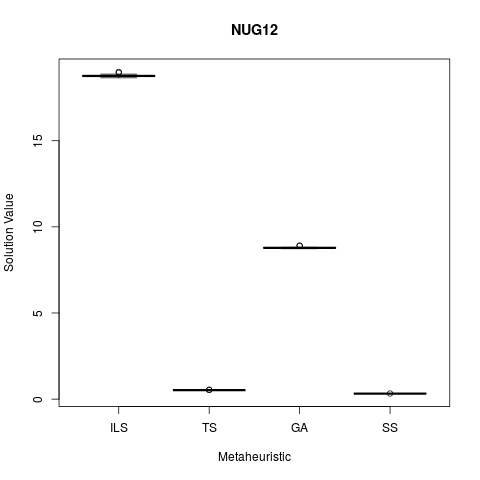
\includegraphics[scale=0.5]{nug12}
    \centering
    \label{fig:boxplot_nug12}
\end{figure}

\begin{figure}[ht]
  \caption{Boxplots de las Soluciones para la instancia Nug14}
  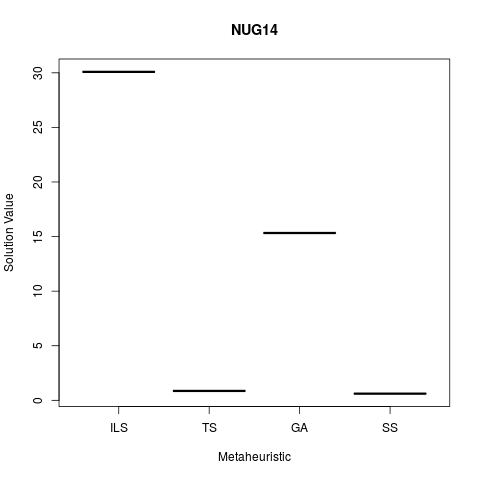
\includegraphics[scale=0.5]{nug14}
    \centering
    \label{fig:boxplot_nug14}
\end{figure}

\begin{figure}[ht]
  \caption{Boxplots de las Soluciones para la instancia Nug15}
  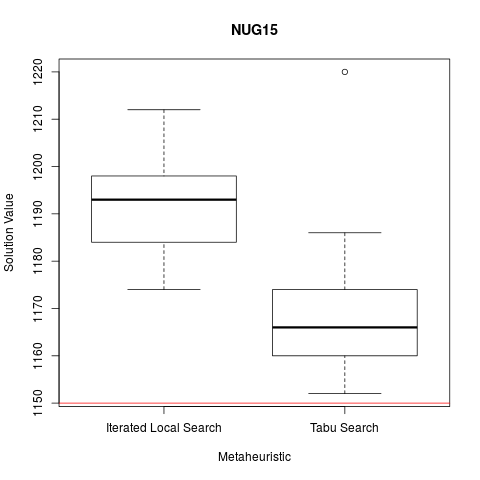
\includegraphics[scale=0.5]{nug15}
    \centering
    \label{fig:boxplot_nug15}
\end{figure}

\begin{figure}[ht]
  \caption{Boxplots de las Soluciones para la instancia Nug16a}
  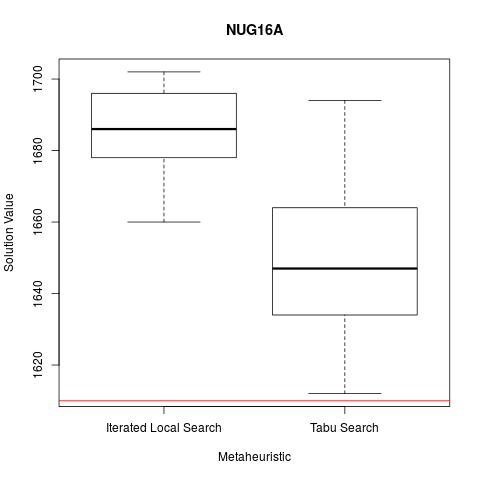
\includegraphics[scale=0.5]{nug16a}
    \centering
    \label{fig:boxplot_nug16a}
\end{figure}

\begin{figure}[ht]
  \caption{Boxplots de las Soluciones para la instancia Nug16b}
  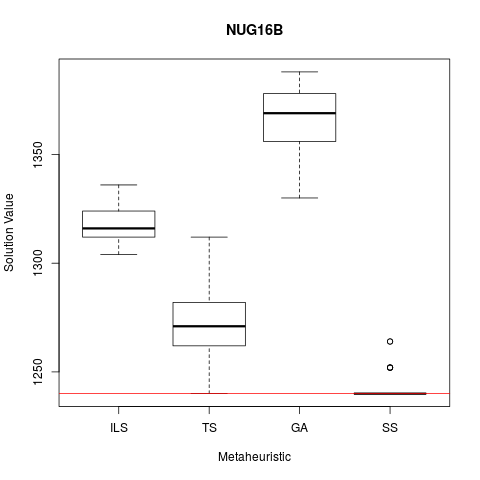
\includegraphics[scale=0.5]{nug16b}
    \centering
    \label{fig:boxplot_nug16b}
\end{figure}

\begin{figure}[ht]
  \caption{Boxplots de las Soluciones para la instancia Nug17}
  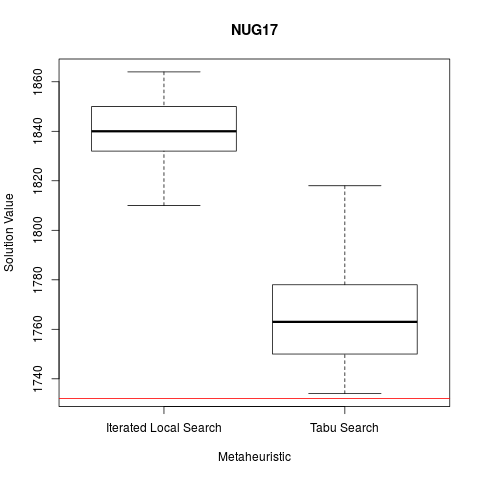
\includegraphics[scale=0.5]{nug17}
    \centering
    \label{fig:boxplot_nug17}
\end{figure}

\begin{figure}[ht]
  \caption{Boxplots de las Soluciones para la instancia Nug18}
  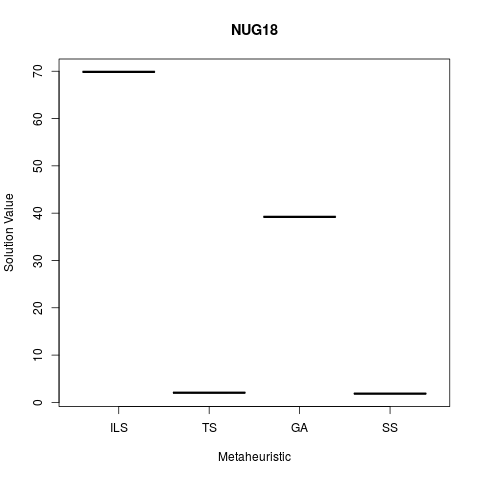
\includegraphics[scale=0.5]{nug18}
    \centering
    \label{fig:boxplot_nug18}
\end{figure}

\begin{figure}[ht]
  \caption{Boxplots de las Soluciones para la instancia Nug20}
  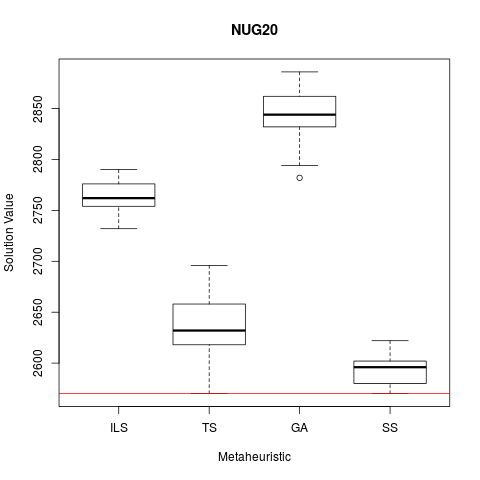
\includegraphics[scale=0.5]{nug20}
    \centering
    \label{fig:boxplot_nug20}
\end{figure}

\begin{figure}[ht]
  \caption{Boxplots de las Soluciones para la instancia Nug21}
  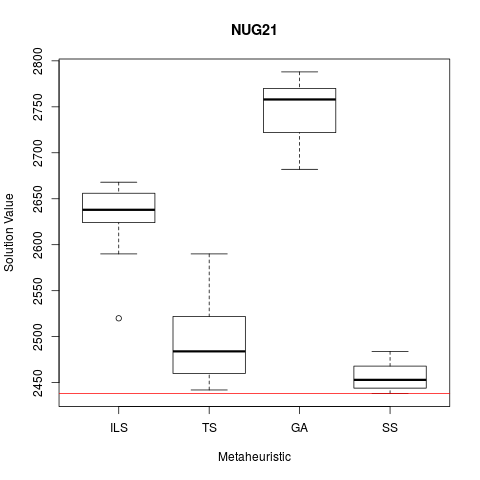
\includegraphics[scale=0.5]{nug21}
    \centering
    \label{fig:boxplot_nug21}
\end{figure}

\begin{figure}[ht]
  \caption{Boxplots de las Soluciones para la instancia Nug22}
  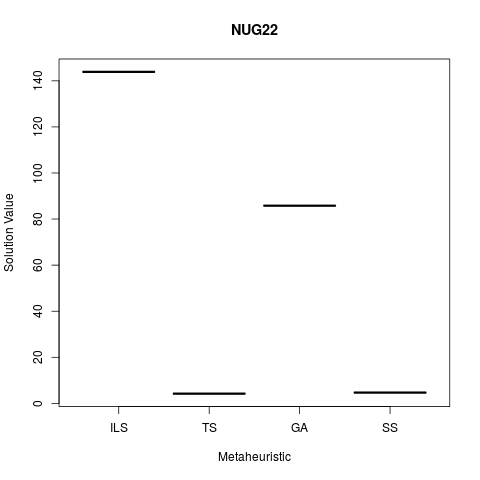
\includegraphics[scale=0.5]{nug22}
    \centering
    \label{fig:boxplot_nug22}
\end{figure}

\begin{figure}[ht]
  \caption{Boxplots de las Soluciones para la instancia Nug24}
  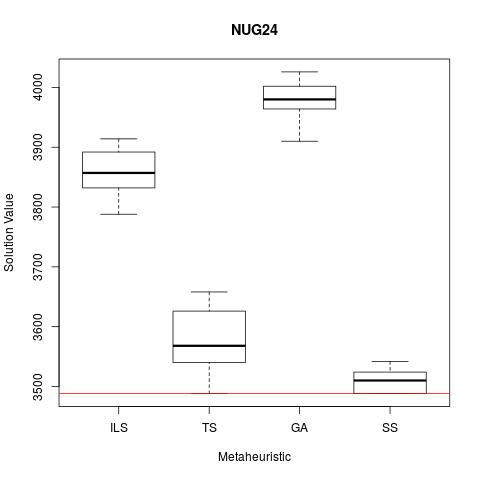
\includegraphics[scale=0.5]{nug24}
    \centering
    \label{fig:boxplot_nug24}
\end{figure}

\begin{figure}[ht]
  \caption{Boxplots de las Soluciones para la instancia Nug25}
  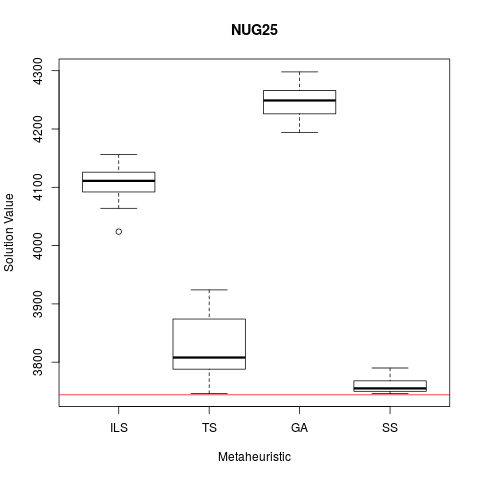
\includegraphics[scale=0.5]{nug25}
    \centering
    \label{fig:boxplot_nug25}
\end{figure}

\begin{figure}[ht]
  \caption{Boxplots de las Soluciones para la instancia Nug27}
  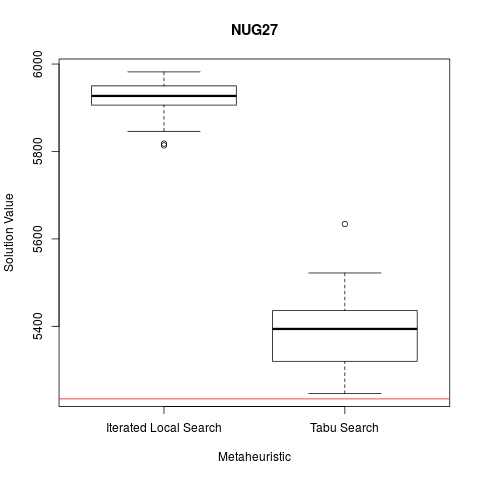
\includegraphics[scale=0.5]{nug27}
    \centering
    \label{fig:boxplot_nug27}
\end{figure}

\begin{figure}[ht]
  \caption{Boxplots de las Soluciones para la instancia Nug28}
  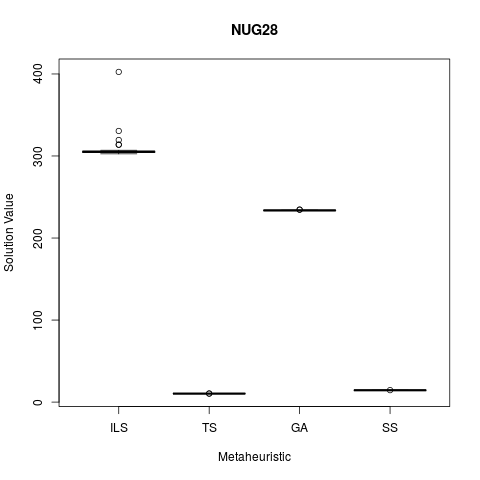
\includegraphics[scale=0.5]{nug28}
    \centering
    \label{fig:boxplot_nug28}
\end{figure}

\begin{figure}[ht]
  \caption{Boxplots de las Soluciones para la instancia Nug30}
  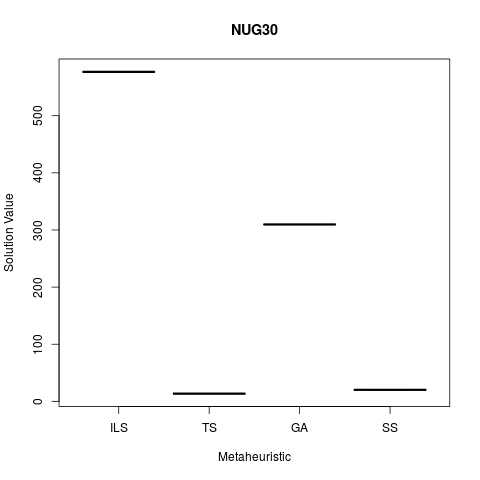
\includegraphics[scale=0.5]{nug30}
    \centering
    \label{fig:boxplot_nug30}
\end{figure}



\begin{table*}[ht]
\centering
\caption{Tabla General}
\label{table:general}
\resizebox{18cm}{!}{
\begin{tabular}{l|l|l|l|l|l|c|c|c|c|c|c|c|c|c|c|c|c|c|c|c|}
\cline{2-21}
                                      & \multicolumn{5}{c|}{ILS}                 & \multicolumn{5}{c|}{TS}            & \multicolumn{5}{c|}{GA}            & \multicolumn{5}{c|}{SS}                  \\ \hline
\multicolumn{1}{|l|}{{\bf Instancia}} & Mín  & Media & Máx  & SD   & ERM         & Mín  & Media & Máx  & SD   & ERM   & Mín  & Media & Máx  & SD   & ERM   & Mín  & Media & Máx  & SD   & ERM         \\ \hline
\multicolumn{1}{|l|}{nug12}           & 578  & 583.3 & 592  & 4.70 & {\bf 0.009} & 578  & 588.1 & 600  & 7.37 & 0.017 & 578  & 604   & 614  & 7.29 & 0.043 & 578  & 583   & 592  & 4.24 & {\bf 0.009} \\ \hline
\multicolumn{1}{|l|}{nug14}           & 1026 & 1046  & 1064 & 10.3 & 0.031       & 1014 & 1043  & 1078 & 15.8 & 0.028 & 1054 & 1079  & 1096 & 11.7 & 0.064 & 1014 & 1021  & 1034 & 6.03 & {\bf 0.006} \\ \hline
\multicolumn{1}{|l|}{nug15}           & 1174 & 1192  & 1212 & 10.4 & 0.036       & 1152 & 1169  & 1220 & 13.9 & 0.016 & 1208 & 1238  & 1262 & 12.6 & 0.076 & 1150 & 1158  & 1166 & 4.91 & {\bf 0.003} \\ \hline
\multicolumn{1}{|l|}{nug16a}          & 1660 & 1685  & 1702 & 11.2 & 0.046       & 1612 & 1650  & 1694 & 20.5 & 0.024 & 1684 & 1735  & 1766 & 20.2 & 0.077 & 1610 & 1617  & 1634 & 8.71 & {\bf 0.004} \\ \hline
\multicolumn{1}{|l|}{nug16b}          & 1304 & 1318  & 1336 & 20.6 & 0.062       & 1240 & 1270  & 1312 & 20.6 & 0.024 & 1330 & 1366  & 1388 & 14.9 & 0.101 & 1240 & 1243  & 1264 & 6.99 & {\bf 0.002} \\ \hline
\multicolumn{1}{|l|}{nug17}           & 1810 & 1839  & 1864 & 13.6 & 0.061       & 1734 & 1764  & 1818 & 17.6 & 0.018 & 1830 & 1888  & 1912 & 18.3 & 0.089 & 1732 & 1742  & 1760 & 7.82 & {\bf 0.005} \\ \hline
\multicolumn{1}{|l|}{nug18}           & 2022 & 2057  & 2084 & 15.3 & 0.065       & 1930 & 1989  & 2010 & 19.6 & 0.021 & 2050 & 2113  & 2148 & 24.1 & 0.094 & 1930 & 1943  & 1958 & 8.93 & {\bf 0.006} \\ \hline
\multicolumn{1}{|l|}{nug20}           & 2732 & 2764  & 2790 & 15.4 & 0.075       & 2570 & 2634  & 2696 & 29.4 & 0.024 & 2782 & 2842  & 2886 & 26.2 & 0.105 & 2570 & 2592  & 2622 & 13.7 & {\bf 0.008} \\ \hline
\multicolumn{1}{|l|}{nug21}           & 2520 & 2635  & 2668 & 29.3 & 0.080       & 2442 & 2495  & 2590 & 40.2 & 0.023 & 2682 & 2747  & 2788 & 29.1 & 0.126 & 2438 & 2457  & 2484 & 14.8 & {\bf 0.007} \\ \hline
\multicolumn{1}{|l|}{nug22}           & 3846 & 3912  & 3960 & 31.2 & 0.087       & 3596 & 3689  & 3854 & 59.9 & 0.025 & 3970 & 4050  & 4114 & 28.3 & 0.126 & 3596 & 3617  & 3652 & 15.5 & {\bf 0.005} \\ \hline
\multicolumn{1}{|l|}{nug24}           & 3788 & 3860  & 3914 & 32.7 & 0.106       & 3488 & 3578  & 3658 & 48.5 & 0.025 & 3910 & 3980  & 4026 & 29.7 & 0.140 & 3488 & 3510  & 3542 & 17.8 & {\bf 0.006} \\ \hline
\multicolumn{1}{|l|}{nug25}           & 4024 & 4108  & 4156 & 29.4 & 0.097       & 3746 & 3823  & 3924 & 50.0 & 0.021 & 4194 & 4248  & 4298 & 25.6 & 0.134 & 3746 & 3760  & 3790 & 13.0 & {\bf 0.004} \\ \hline
\multicolumn{1}{|l|}{nug27}           & 5814 & 5920  & 5982 & 44.5 & 0.131       & 5246 & 5389  & 5634 & 80.1 & 0.029 & 5850 & 5958  & 6044 & 50.5 & 0.138 & 5234 & 5276  & 5338 & 31.2 & {\bf 0.008} \\ \hline
\multicolumn{1}{|l|}{nug28}           & 5768 & 5860  & 5922 & 36.4 & 0.134       & 5190 & 5301  & 5408 & 58.5 & 0.026 & 5798 & 5926  & 5988 & 45.4 & 0.147 & 5166 & 5224  & 5266 & 24.3 & {\bf 0.011} \\ \hline
\multicolumn{1}{|l|}{nug30}           & 6688 & 6846  & 6914 & 49.2 & 0.117       & 6156 & 6283  & 6490 & 83.4 & 0.025 & 6880 & 7059  & 7140 & 48.7 & 0.152 & 6148 & 6185  & 6242 & 22.1 & {\bf 0.009} \\ \hline
\end{tabular}
}
\end{table*}

%
%Bla.

\end{document}
